\documentclass[xcolor=dvipsnames]{beamer}\usepackage[]{graphicx}\usepackage[]{color}
%% maxwidth is the original width if it is less than linewidth
%% otherwise use linewidth (to make sure the graphics do not exceed the margin)
\makeatletter
\def\maxwidth{ %
  \ifdim\Gin@nat@width>\linewidth
    \linewidth
  \else
    \Gin@nat@width
  \fi
}
\makeatother

\definecolor{fgcolor}{rgb}{0.345, 0.345, 0.345}
\newcommand{\hlnum}[1]{\textcolor[rgb]{0.686,0.059,0.569}{#1}}%
\newcommand{\hlstr}[1]{\textcolor[rgb]{0.192,0.494,0.8}{#1}}%
\newcommand{\hlcom}[1]{\textcolor[rgb]{0.678,0.584,0.686}{\textit{#1}}}%
\newcommand{\hlopt}[1]{\textcolor[rgb]{0,0,0}{#1}}%
\newcommand{\hlstd}[1]{\textcolor[rgb]{0.345,0.345,0.345}{#1}}%
\newcommand{\hlkwa}[1]{\textcolor[rgb]{0.161,0.373,0.58}{\textbf{#1}}}%
\newcommand{\hlkwb}[1]{\textcolor[rgb]{0.69,0.353,0.396}{#1}}%
\newcommand{\hlkwc}[1]{\textcolor[rgb]{0.333,0.667,0.333}{#1}}%
\newcommand{\hlkwd}[1]{\textcolor[rgb]{0.737,0.353,0.396}{\textbf{#1}}}%

\usepackage{framed}
\makeatletter
\newenvironment{kframe}{%
 \def\at@end@of@kframe{}%
 \ifinner\ifhmode%
  \def\at@end@of@kframe{\end{minipage}}%
  \begin{minipage}{\columnwidth}%
 \fi\fi%
 \def\FrameCommand##1{\hskip\@totalleftmargin \hskip-\fboxsep
 \colorbox{shadecolor}{##1}\hskip-\fboxsep
     % There is no \\@totalrightmargin, so:
     \hskip-\linewidth \hskip-\@totalleftmargin \hskip\columnwidth}%
 \MakeFramed {\advance\hsize-\width
   \@totalleftmargin\z@ \linewidth\hsize
   \@setminipage}}%
 {\par\unskip\endMakeFramed%
 \at@end@of@kframe}
\makeatother

\definecolor{shadecolor}{rgb}{.97, .97, .97}
\definecolor{messagecolor}{rgb}{0, 0, 0}
\definecolor{warningcolor}{rgb}{1, 0, 1}
\definecolor{errorcolor}{rgb}{1, 0, 0}
\newenvironment{knitrout}{}{} % an empty environment to be redefined in TeX

\usepackage{alltt}
%%\usepackage[dvipsnames]{xcolor}

\usefonttheme[onlymath]{serif}

\setbeamercolor{title}{fg=black}
\setbeamercolor{frametitle}{fg=black}

\setbeamertemplate{itemize items}[circle] 
\setbeamercolor{itemize item}{fg=black}
\IfFileExists{upquote.sty}{\usepackage{upquote}}{} 
\begin{document}

\title{Another View of Ordinary Regression}
\author{PirateGruntTV}

\maketitle

% very important to use option [fragile] for frames containing code output!




\begin{frame}[fragile]{Another view of linear regression}
\begin{knitrout}
\definecolor{shadecolor}{rgb}{0.969, 0.969, 0.969}\color{fgcolor}\begin{kframe}
\begin{alltt}
\hlkwd{set.seed}\hlstd{(}\hlnum{1234}\hlstd{)}
\hlstd{N} \hlkwb{=} \hlnum{100}
\hlstd{e} \hlkwb{=} \hlkwd{rnorm}\hlstd{(N,} \hlkwc{mean} \hlstd{=} \hlnum{0}\hlstd{,} \hlkwc{sd} \hlstd{=} \hlnum{1}\hlstd{)}
\hlstd{lnLike} \hlkwb{=} \hlkwa{function}\hlstd{(}\hlkwc{x}\hlstd{,} \hlkwc{mu}\hlstd{,} \hlkwc{sigma}\hlstd{) \{}
    \hlstd{n} \hlkwb{=} \hlkwd{length}\hlstd{(x)}
    \hlstd{lnLike} \hlkwb{=} \hlopt{-}\hlstd{n}\hlopt{/}\hlnum{2} \hlopt{*} \hlkwd{log}\hlstd{(}\hlnum{2} \hlopt{*} \hlstd{pi)}
    \hlstd{lnLike} \hlkwb{=} \hlstd{lnLike} \hlopt{-} \hlstd{n}\hlopt{/}\hlnum{2} \hlopt{*} \hlkwd{log}\hlstd{(sigma}\hlopt{^}\hlnum{2}\hlstd{)}
    \hlstd{lnLike} \hlkwb{=} \hlstd{lnLike} \hlopt{-} \hlnum{1}\hlopt{/}\hlstd{(}\hlnum{2} \hlopt{*} \hlstd{sigma}\hlopt{^}\hlnum{2}\hlstd{)} \hlopt{*} \hlkwd{sum}\hlstd{((x} \hlopt{-}
        \hlstd{mu)}\hlopt{^}\hlnum{2}\hlstd{)}
    \hlstd{lnLike}
\hlstd{\}}
\end{alltt}
\end{kframe}
\end{knitrout}

\end{frame}

\begin{frame}[fragile]
\begin{knitrout}
\definecolor{shadecolor}{rgb}{0.969, 0.969, 0.969}\color{fgcolor}\begin{kframe}
\begin{alltt}
\hlstd{testMu} \hlkwb{=} \hlkwd{seq}\hlstd{(}\hlopt{-}\hlnum{0.5}\hlstd{,} \hlnum{0.5}\hlstd{,} \hlkwc{length.out} \hlstd{=} \hlnum{100}\hlstd{)}
\hlstd{likelihood} \hlkwb{=} \hlkwd{sapply}\hlstd{(testMu, lnLike,} \hlkwc{x} \hlstd{= e,}
    \hlkwc{sigma} \hlstd{=} \hlnum{1}\hlstd{)}
\hlstd{testMu[likelihood} \hlopt{==} \hlkwd{max}\hlstd{(likelihood)]}
\end{alltt}
\begin{verbatim}
## [1] -0.1566
\end{verbatim}
\end{kframe}
\end{knitrout}

\end{frame}

\begin{frame}[fragile]
\begin{knitrout}
\definecolor{shadecolor}{rgb}{0.969, 0.969, 0.969}\color{fgcolor}\begin{kframe}
\begin{alltt}
\hlkwd{plot}\hlstd{(likelihood} \hlopt{~} \hlstd{testMu,} \hlkwc{pch} \hlstd{=} \hlnum{19}\hlstd{)}
\hlkwd{abline}\hlstd{(}\hlkwc{v} \hlstd{=} \hlnum{0}\hlstd{)}
\hlkwd{abline}\hlstd{(}\hlkwc{v} \hlstd{= testMu[likelihood} \hlopt{==} \hlkwd{max}\hlstd{(likelihood)])}
\end{alltt}
\end{kframe}
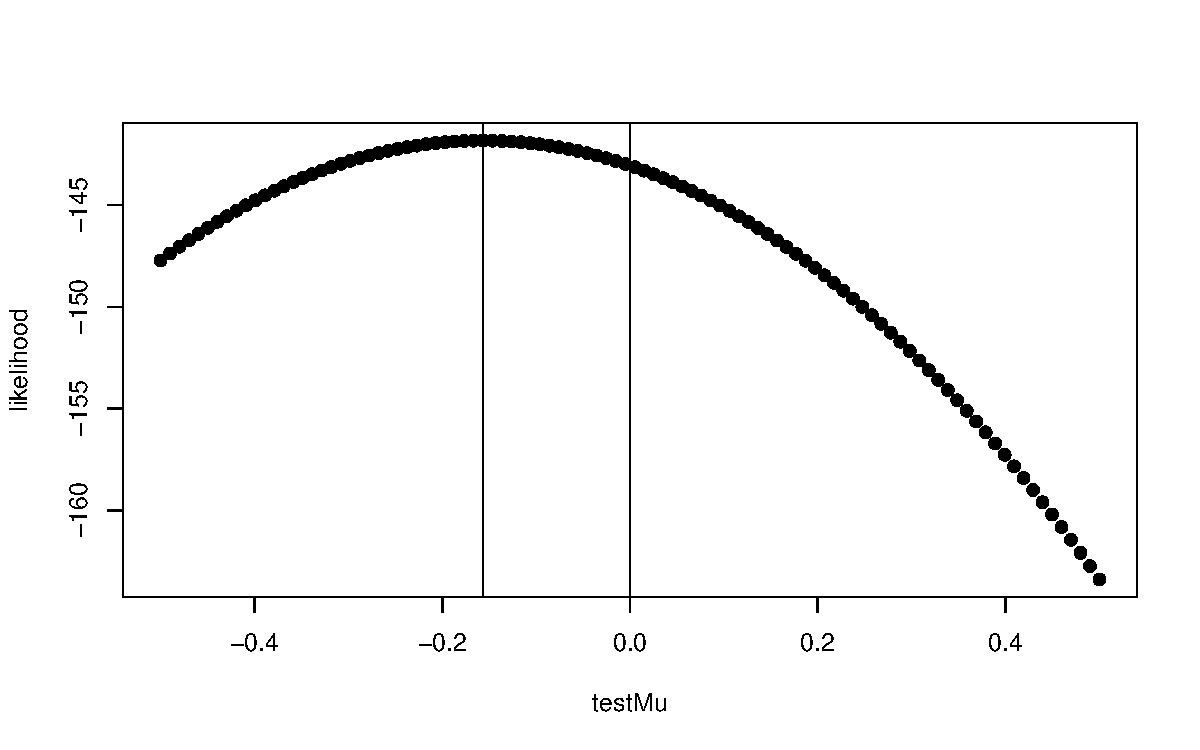
\includegraphics[width=\maxwidth]{figure/unnamed-chunk-1} 

\end{knitrout}

\end{frame}

\begin{frame}[fragile]
\begin{knitrout}
\definecolor{shadecolor}{rgb}{0.969, 0.969, 0.969}\color{fgcolor}\begin{kframe}
\begin{alltt}
\hlstd{testSigma} \hlkwb{=} \hlkwd{seq}\hlstd{(}\hlnum{0.5}\hlstd{,} \hlnum{1.5}\hlstd{,} \hlkwc{length.out} \hlstd{=} \hlnum{100}\hlstd{)}
\hlstd{likelihood} \hlkwb{=} \hlkwd{sapply}\hlstd{(testSigma, lnLike,} \hlkwc{x} \hlstd{= e,}
    \hlkwc{mu} \hlstd{=} \hlnum{0}\hlstd{)}
\hlstd{testSigma[likelihood} \hlopt{==} \hlkwd{max}\hlstd{(likelihood)]}
\end{alltt}
\begin{verbatim}
## [1] 1.015
\end{verbatim}
\end{kframe}
\end{knitrout}

\end{frame}

\begin{frame}[fragile]
\begin{knitrout}
\definecolor{shadecolor}{rgb}{0.969, 0.969, 0.969}\color{fgcolor}\begin{kframe}
\begin{alltt}
\hlkwd{plot}\hlstd{(likelihood} \hlopt{~} \hlstd{testSigma,} \hlkwc{pch} \hlstd{=} \hlnum{19}\hlstd{)}
\hlkwd{abline}\hlstd{(}\hlkwc{v} \hlstd{=} \hlnum{1}\hlstd{)}
\hlkwd{abline}\hlstd{(}\hlkwc{v} \hlstd{= testSigma[likelihood} \hlopt{==} \hlkwd{max}\hlstd{(likelihood)])}
\end{alltt}
\end{kframe}
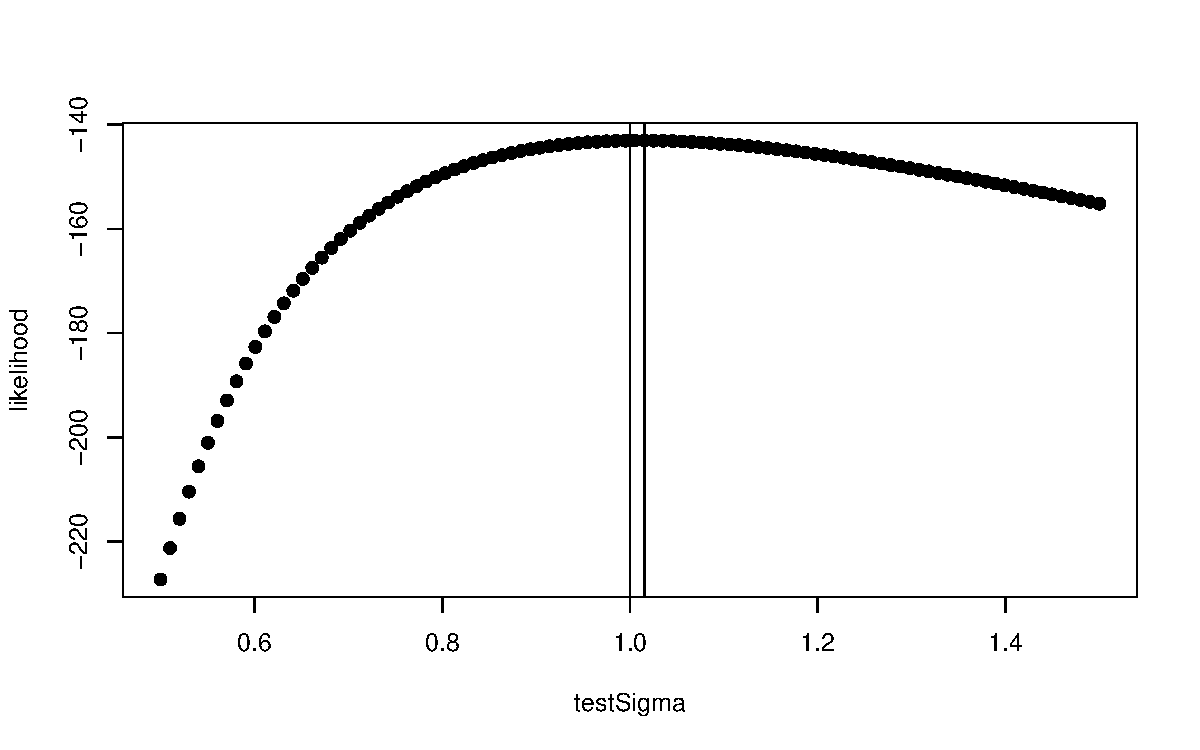
\includegraphics[width=\maxwidth]{figure/PlotSigma} 

\end{knitrout}

\end{frame}

\begin{frame}[fragile]
\begin{knitrout}
\definecolor{shadecolor}{rgb}{0.969, 0.969, 0.969}\color{fgcolor}\begin{kframe}
\begin{alltt}
\hlstd{params} \hlkwb{=} \hlkwd{expand.grid}\hlstd{(}\hlkwc{mu} \hlstd{= testMu,} \hlkwc{sigma} \hlstd{= testSigma)}
\hlstd{params}\hlopt{$}\hlstd{Likelihood} \hlkwb{=} \hlkwd{mapply}\hlstd{(lnLike, params}\hlopt{$}\hlstd{mu,}
    \hlstd{params}\hlopt{$}\hlstd{sigma,} \hlkwc{MoreArgs} \hlstd{=} \hlkwd{list}\hlstd{(}\hlkwc{x} \hlstd{= e))}
\hlstd{z} \hlkwb{=} \hlkwd{matrix}\hlstd{(params}\hlopt{$}\hlstd{Likelihood,} \hlkwd{length}\hlstd{(testMu),}
    \hlkwd{length}\hlstd{(testSigma))}
\end{alltt}
\end{kframe}
\end{knitrout}

\end{frame}

\begin{frame}[fragile]
\begin{knitrout}
\definecolor{shadecolor}{rgb}{0.969, 0.969, 0.969}\color{fgcolor}\begin{kframe}
\begin{alltt}
\hlkwd{filled.contour}\hlstd{(}\hlkwc{x} \hlstd{= testMu,} \hlkwc{y} \hlstd{= testSigma,}
    \hlkwc{z} \hlstd{= z,} \hlkwc{color.palette} \hlstd{= heat.colors,} \hlkwc{xlab} \hlstd{=} \hlstr{"mu"}\hlstd{,}
    \hlkwc{ylab} \hlstd{=} \hlstr{"sigma"}\hlstd{)}
\end{alltt}
\end{kframe}
\end{knitrout}

\end{frame}

\begin{frame}[fragile]
\begin{knitrout}
\definecolor{shadecolor}{rgb}{0.969, 0.969, 0.969}\color{fgcolor}
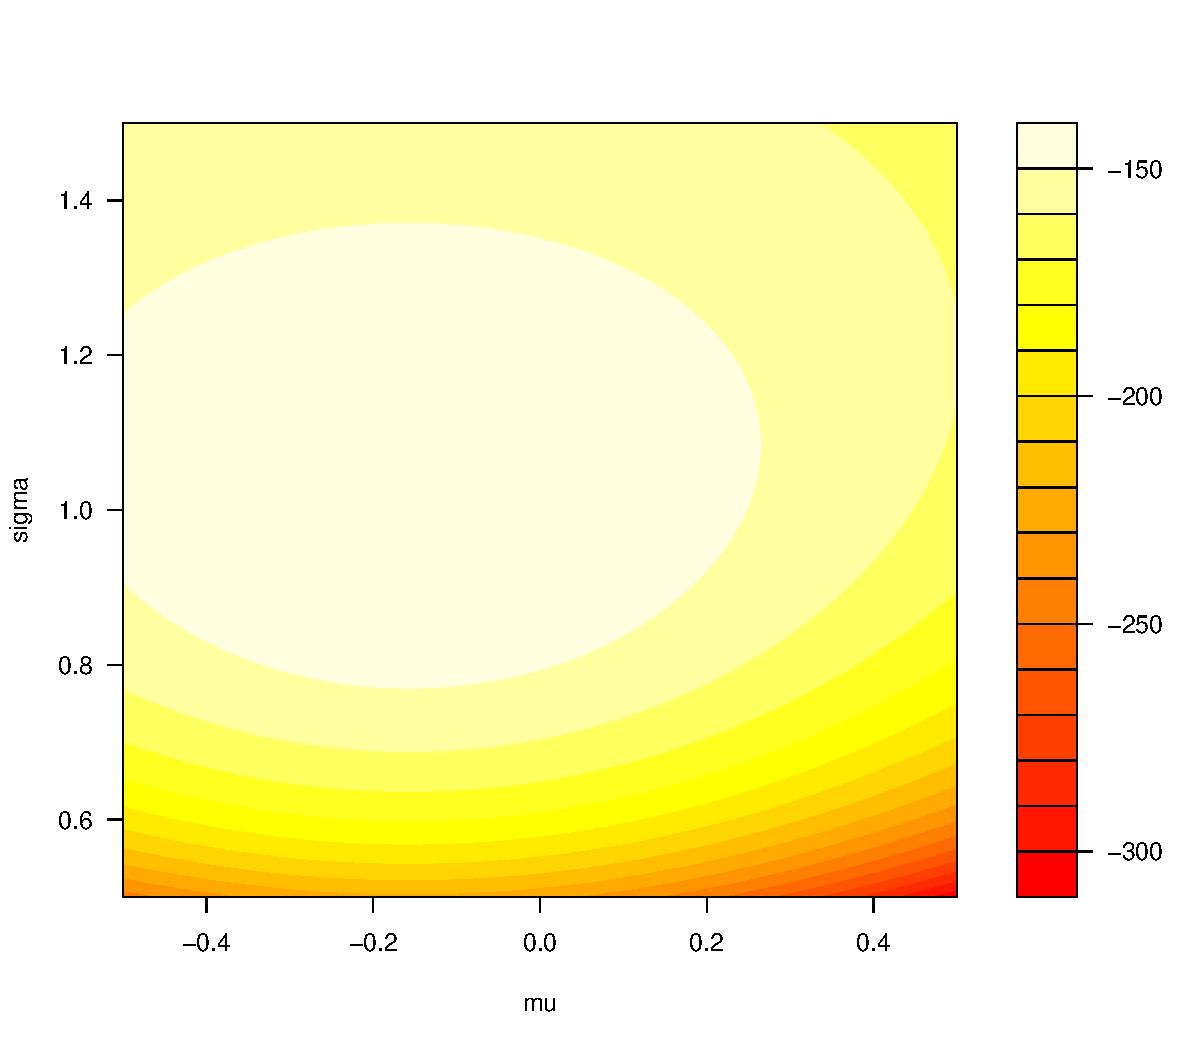
\includegraphics[width=\maxwidth]{figure/TwoDimPlotOutput} 

\end{knitrout}

\end{frame}

\begin{frame}[fragile]{Optimize for both parameters}
\begin{knitrout}
\definecolor{shadecolor}{rgb}{0.969, 0.969, 0.969}\color{fgcolor}\begin{kframe}
\begin{alltt}
\hlstd{lnLike2} \hlkwb{=} \hlkwa{function}\hlstd{(}\hlkwc{x}\hlstd{,} \hlkwc{par}\hlstd{) \{}
    \hlstd{mu} \hlkwb{=} \hlstd{par[}\hlnum{1}\hlstd{]}
    \hlstd{sigma} \hlkwb{=} \hlstd{par[}\hlnum{2}\hlstd{]}
    \hlkwd{lnLike}\hlstd{(x, mu, sigma)}
\hlstd{\}}
\hlstd{optimFit} \hlkwb{=} \hlkwd{optim}\hlstd{(}\hlkwc{par} \hlstd{=} \hlkwd{c}\hlstd{(}\hlopt{-}\hlnum{1}\hlstd{,} \hlnum{4}\hlstd{),} \hlkwc{fn} \hlstd{= lnLike2,}
    \hlkwc{control} \hlstd{=} \hlkwd{list}\hlstd{(}\hlkwc{fnscale} \hlstd{=} \hlopt{-}\hlnum{1}\hlstd{),} \hlkwc{x} \hlstd{= e)}
\hlstd{optimFit}\hlopt{$}\hlstd{par}
\end{alltt}
\begin{verbatim}
## [1] -0.1566  0.9994
\end{verbatim}
\end{kframe}
\end{knitrout}

\end{frame}

\begin{frame}[fragile]{Add a constant term to the normal variable e}
\begin{knitrout}
\definecolor{shadecolor}{rgb}{0.969, 0.969, 0.969}\color{fgcolor}\begin{kframe}
\begin{alltt}
\hlstd{B0} \hlkwb{=} \hlnum{5}
\hlstd{Y} \hlkwb{=} \hlstd{B0} \hlopt{+} \hlstd{e}
\end{alltt}
\end{kframe}
\end{knitrout}

\end{frame}
 
\begin{frame}[fragile]{This is equivalent to lm}
\begin{knitrout}
\definecolor{shadecolor}{rgb}{0.969, 0.969, 0.969}\color{fgcolor}\begin{kframe}
\begin{alltt}
\hlstd{optimFit} \hlkwb{=} \hlkwd{optim}\hlstd{(}\hlkwc{par} \hlstd{=} \hlkwd{c}\hlstd{(}\hlopt{-}\hlnum{1}\hlstd{,} \hlnum{4}\hlstd{),} \hlkwc{fn} \hlstd{= lnLike2,}
    \hlkwc{control} \hlstd{=} \hlkwd{list}\hlstd{(}\hlkwc{fnscale} \hlstd{=} \hlopt{-}\hlnum{1}\hlstd{),} \hlkwc{x} \hlstd{= Y)}
\hlstd{optimFit}\hlopt{$}\hlstd{par[[}\hlnum{1}\hlstd{]]}
\end{alltt}
\begin{verbatim}
## [1] 4.843
\end{verbatim}
\begin{alltt}
\hlstd{lmFit} \hlkwb{=} \hlkwd{lm}\hlstd{(Y} \hlopt{~} \hlnum{1}\hlstd{)}
\hlstd{lmFit}\hlopt{$}\hlstd{coefficients[[}\hlnum{1}\hlstd{]]}
\end{alltt}
\begin{verbatim}
## [1] 4.843
\end{verbatim}
\end{kframe}
\end{knitrout}

\end{frame}

\begin{frame}[fragile]{Now add a slope}
\begin{knitrout}
\definecolor{shadecolor}{rgb}{0.969, 0.969, 0.969}\color{fgcolor}\begin{kframe}
\begin{alltt}
\hlstd{X} \hlkwb{=} \hlkwd{as.double}\hlstd{(}\hlnum{1}\hlopt{:}\hlkwd{length}\hlstd{(e))}
\hlstd{B1} \hlkwb{=} \hlnum{1.5}
\hlstd{Y} \hlkwb{=} \hlstd{B0} \hlopt{+} \hlstd{B1} \hlopt{*} \hlstd{X} \hlopt{+} \hlstd{e}
\hlstd{lnLike3} \hlkwb{=} \hlkwa{function}\hlstd{(}\hlkwc{par}\hlstd{,} \hlkwc{Y}\hlstd{,} \hlkwc{X}\hlstd{) \{}
    \hlstd{B0} \hlkwb{=} \hlstd{par[}\hlnum{1}\hlstd{]}
    \hlstd{B1} \hlkwb{=} \hlstd{par[}\hlnum{2}\hlstd{]}
    \hlstd{sigma} \hlkwb{=} \hlstd{par[}\hlnum{3}\hlstd{]}
    \hlstd{x} \hlkwb{=} \hlstd{Y} \hlopt{-} \hlstd{B0} \hlopt{-} \hlstd{B1} \hlopt{*} \hlstd{X}
    \hlstd{mu} \hlkwb{=} \hlnum{0}
    \hlkwd{lnLike}\hlstd{(x, mu, sigma)}
\hlstd{\}}
\end{alltt}
\end{kframe}
\end{knitrout}

\end{frame}

\begin{frame}[fragile]
\begin{knitrout}
\definecolor{shadecolor}{rgb}{0.969, 0.969, 0.969}\color{fgcolor}\begin{kframe}
\begin{alltt}
\hlstd{optimFit} \hlkwb{=} \hlkwd{optim}\hlstd{(}\hlkwc{par} \hlstd{=} \hlkwd{c}\hlstd{(}\hlnum{4}\hlstd{,} \hlnum{1}\hlstd{,} \hlnum{1}\hlstd{),} \hlkwc{fn} \hlstd{= lnLike3,}
    \hlkwc{control} \hlstd{=} \hlkwd{list}\hlstd{(}\hlkwc{fnscale} \hlstd{=} \hlopt{-}\hlnum{1}\hlstd{),} \hlkwc{Y} \hlstd{= Y,}
    \hlkwc{X} \hlstd{= X)}
\hlstd{optimFit}\hlopt{$}\hlstd{par[}\hlnum{1}\hlopt{:}\hlnum{2}\hlstd{]}
\end{alltt}
\begin{verbatim}
## [1] 4.404 1.509
\end{verbatim}
\begin{alltt}
\hlstd{lmFit} \hlkwb{=} \hlkwd{lm}\hlstd{(Y} \hlopt{~} \hlnum{1} \hlopt{+} \hlstd{X)}
\hlstd{lmFit}\hlopt{$}\hlstd{coefficients}
\end{alltt}
\begin{verbatim}
## (Intercept)           X 
##       4.406       1.509
\end{verbatim}
\end{kframe}
\end{knitrout}

\end{frame}

\begin{frame}
Why does this matter?
\end{frame}

\begin{frame}
pirategrunt.com
\end{frame}

\end{document}
